% Appendix A: Feature Importance Tables

\chapter{Feature Importance Tables}
\label{app:feature-importance}

\section{Overview}

This appendix presents the top-20 most important features for each experimental condition, as determined by model-native importance measures:

\begin{itemize}
    \item \textbf{Logistic Regression:} Absolute coefficient values
    \item \textbf{Random Forest:} Gini importance (mean decrease in impurity)
\end{itemize}

\section{Dataset A --- ReadText Task}

\subsection{Random Forest --- Top 20 Features}

\begin{table}[H]
\centering
\begin{tabular}{@{}clcc@{}}
\toprule
\textbf{Rank} & \textbf{Feature} & \textbf{Importance} & \textbf{Std} \\
\midrule
1 & f0\_max & 0.052 & 0.019 \\
2 & delta\_mfcc\_2\_mean & 0.039 & 0.018 \\
3 & f3\_std & 0.038 & 0.011 \\
4 & autocorr\_harmonicity & 0.038 & 0.017 \\
5 & intensity\_mean & 0.035 & 0.021 \\
6 & f0\_mean & 0.032 & 0.012 \\
7 & shimmer\_apq3 & 0.032 & 0.013 \\
8 & mfcc\_12\_mean & 0.031 & 0.007 \\
9 & f1\_std & 0.031 & 0.022 \\
10 & mfcc\_6\_mean & 0.030 & 0.024 \\
\bottomrule
\end{tabular}
\caption{Random Forest feature importance --- ReadText (top 10)}
\label{tab:rf-readtext-importance}
\end{table}

\subsection{Logistic Regression --- Top 20 Features}

\begin{table}[H]
\centering
\begin{tabular}{@{}clcc@{}}
\toprule
\textbf{Rank} & \textbf{Feature} & \textbf{|Coefficient|} & \textbf{Std} \\
\midrule
1 & f0\_max & 0.754 & 0.203 \\
2 & hnr\_mean & 0.649 & 0.178 \\
3 & shimmer\_apq11 & 0.553 & 0.145 \\
4 & delta\_mfcc\_4\_mean & 0.496 & 0.163 \\
5 & delta\_mfcc\_2\_mean & 0.492 & 0.103 \\
6 & delta\_mfcc\_1\_mean & 0.474 & 0.273 \\
7 & mfcc\_5\_mean & 0.470 & 0.127 \\
8 & mfcc\_4\_mean & 0.426 & 0.233 \\
9 & mfcc\_10\_mean & 0.418 & 0.221 \\
10 & mfcc\_11\_mean & 0.388 & 0.192 \\
\bottomrule
\end{tabular}
\caption{Logistic Regression feature importance --- ReadText (top 10)}
\label{tab:lr-readtext-importance}
\end{table}

\begin{figure}[H]
    \centering
    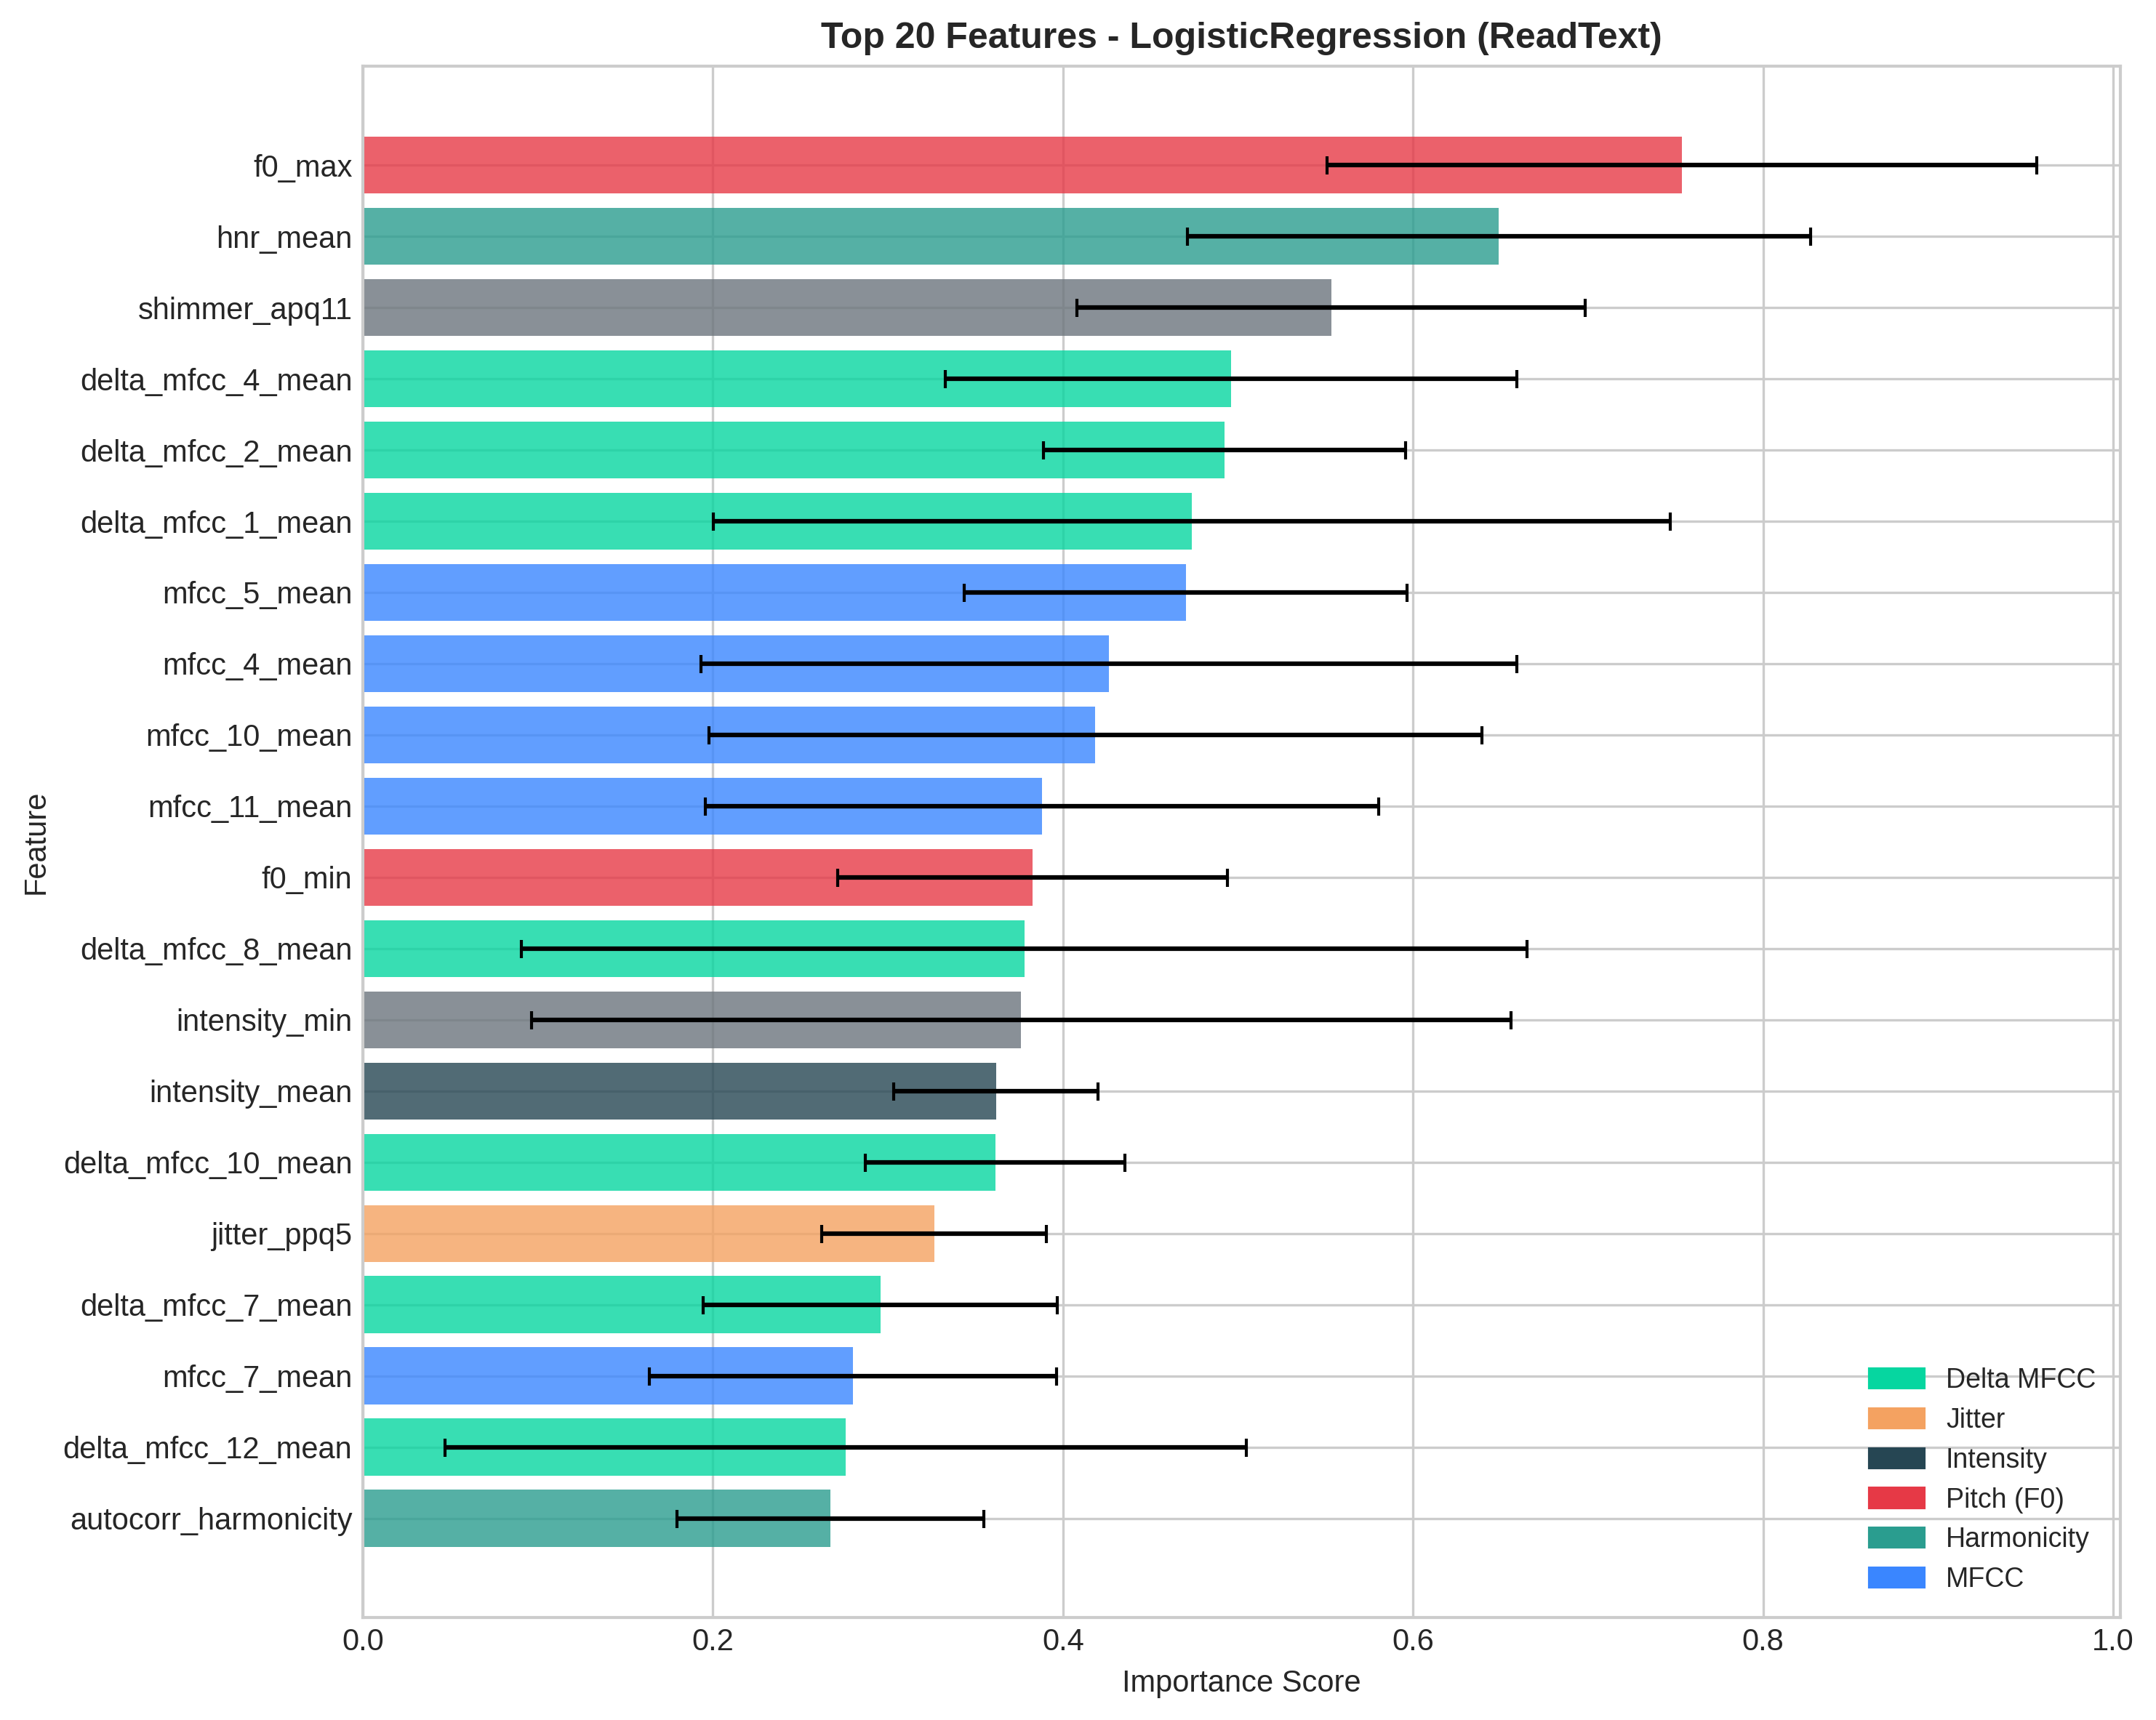
\includegraphics[width=0.8\textwidth]{figures/fig_imp_readtext_lr.png}
    \caption{Logistic Regression coefficient magnitudes (ReadText)}
    \label{fig:imp-readtext-lr}
\end{figure}

\subsection{Gradient Boosting --- Top 10 Features}

\begin{table}[H]
\centering
\begin{tabular}{@{}clcc@{}}
\toprule
\textbf{Rank} & \textbf{Feature} & \textbf{Importance} & \textbf{Std} \\
\midrule
1 & f0\_max & 0.229 & 0.179 \\
2 & mfcc\_4\_mean & 0.084 & 0.187 \\
3 & f1\_std & 0.080 & 0.178 \\
4 & mfcc\_6\_mean & 0.066 & 0.143 \\
5 & intensity\_min & 0.064 & 0.122 \\
6 & mfcc\_2\_mean & 0.060 & 0.133 \\
7 & f0\_std & 0.055 & 0.081 \\
8 & f3\_std & 0.054 & 0.070 \\
9 & delta\_mfcc\_10\_mean & 0.047 & 0.104 \\
10 & delta\_mfcc\_2\_mean & 0.041 & 0.083 \\
\bottomrule
\end{tabular}
\caption{Gradient Boosting feature importance --- ReadText (top 10)}
\label{tab:gb-readtext-importance}
\end{table}

\begin{figure}[H]
    \centering
    
\includegraphics[width=0.8\textwidth]{fig_imp_readtext_gb.png}
    \caption{Gradient Boosting feature importances (ReadText). F0 max dominates strongly ($0.229 \pm 0.179$), consistent with pitch dysregulation in PD.}
    \label{fig:imp-readtext-gb}
\end{figure}

\subsection{XGBoost --- Top 10 Features}

\begin{table}[H]
\centering
\begin{tabular}{@{}clcc@{}}
\toprule
\textbf{Rank} & \textbf{Feature} & \textbf{Importance} & \textbf{Std} \\
\midrule
1 & f0\_max & 0.083 & 0.028 \\
2 & intensity\_min & 0.064 & 0.063 \\
3 & f0\_mean & 0.063 & 0.044 \\
4 & f3\_std & 0.061 & 0.044 \\
5 & intensity\_mean & 0.051 & 0.047 \\
6 & delta\_mfcc\_10\_mean & 0.041 & 0.037 \\
7 & f1\_std & 0.041 & 0.075 \\
8 & delta\_mfcc\_2\_mean & 0.038 & 0.028 \\
9 & mfcc\_3\_mean & 0.033 & 0.023 \\
10 & mfcc\_11\_mean & 0.031 & 0.040 \\
\bottomrule
\end{tabular}
\caption{XGBoost feature importance --- ReadText (top 10)}
\label{tab:xgb-readtext-importance}
\end{table}

\begin{figure}[H]
    \centering
    
\includegraphics[width=0.8\textwidth]{fig_imp_readtext_xgb.png}
    \caption{XGBoost feature importances (ReadText). Importance is more distributed than Gradient Boosting, with F0 and intensity features sharing dominance.}
    \label{fig:imp-readtext-xgb}
\end{figure}

\section{Dataset A --- SpontaneousDialogue Task}

\subsection{Random Forest --- Top 20 Features}

\begin{table}[H]
\centering
\begin{tabular}{@{}clcc@{}}
\toprule
\textbf{Rank} & \textbf{Feature} & \textbf{Importance} & \textbf{Std} \\
\midrule
1 & mfcc\_5\_mean & 0.080 & 0.022 \\
2 & shimmer\_apq11 & 0.069 & 0.007 \\
3 & delta\_mfcc\_8\_mean & 0.051 & 0.015 \\
4 & jitter\_local & 0.041 & 0.012 \\
5 & delta\_mfcc\_2\_mean & 0.040 & 0.018 \\
6 & autocorr\_harmonicity & 0.037 & 0.011 \\
7 & shimmer\_local & 0.036 & 0.017 \\
8 & mfcc\_1\_mean & 0.034 & 0.010 \\
9 & f0\_std & 0.032 & 0.022 \\
10 & f0\_mean & 0.031 & 0.013 \\
\bottomrule
\end{tabular}
\caption{Random Forest feature importance --- SpontaneousDialogue (top 10)}
\label{tab:rf-spontaneous-importance}
\end{table}

\subsection{Logistic Regression --- Top 10 Features}

\begin{table}[H]
\centering
\begin{tabular}{@{}clcc@{}}
\toprule
\textbf{Rank} & \textbf{Feature} & \textbf{|Coefficient|} & \textbf{Std} \\
\midrule
1 & mfcc\_5\_mean & 0.722 & 0.039 \\
2 & delta\_mfcc\_8\_mean & 0.615 & 0.121 \\
3 & shimmer\_apq11 & 0.559 & 0.136 \\
4 & delta\_mfcc\_2\_mean & 0.493 & 0.196 \\
5 & intensity\_min & 0.459 & 0.170 \\
6 & mfcc\_3\_mean & 0.388 & 0.271 \\
7 & delta\_mfcc\_11\_mean & 0.381 & 0.102 \\
8 & delta\_mfcc\_7\_mean & 0.380 & 0.150 \\
9 & hnr\_mean & 0.379 & 0.175 \\
10 & delta\_mfcc\_1\_mean & 0.352 & 0.123 \\
\bottomrule
\end{tabular}
\caption{Logistic Regression feature importance --- SpontaneousDialogue (top 10)}
\label{tab:lr-spontaneous-importance}
\end{table}

\begin{figure}[H]
    \centering
    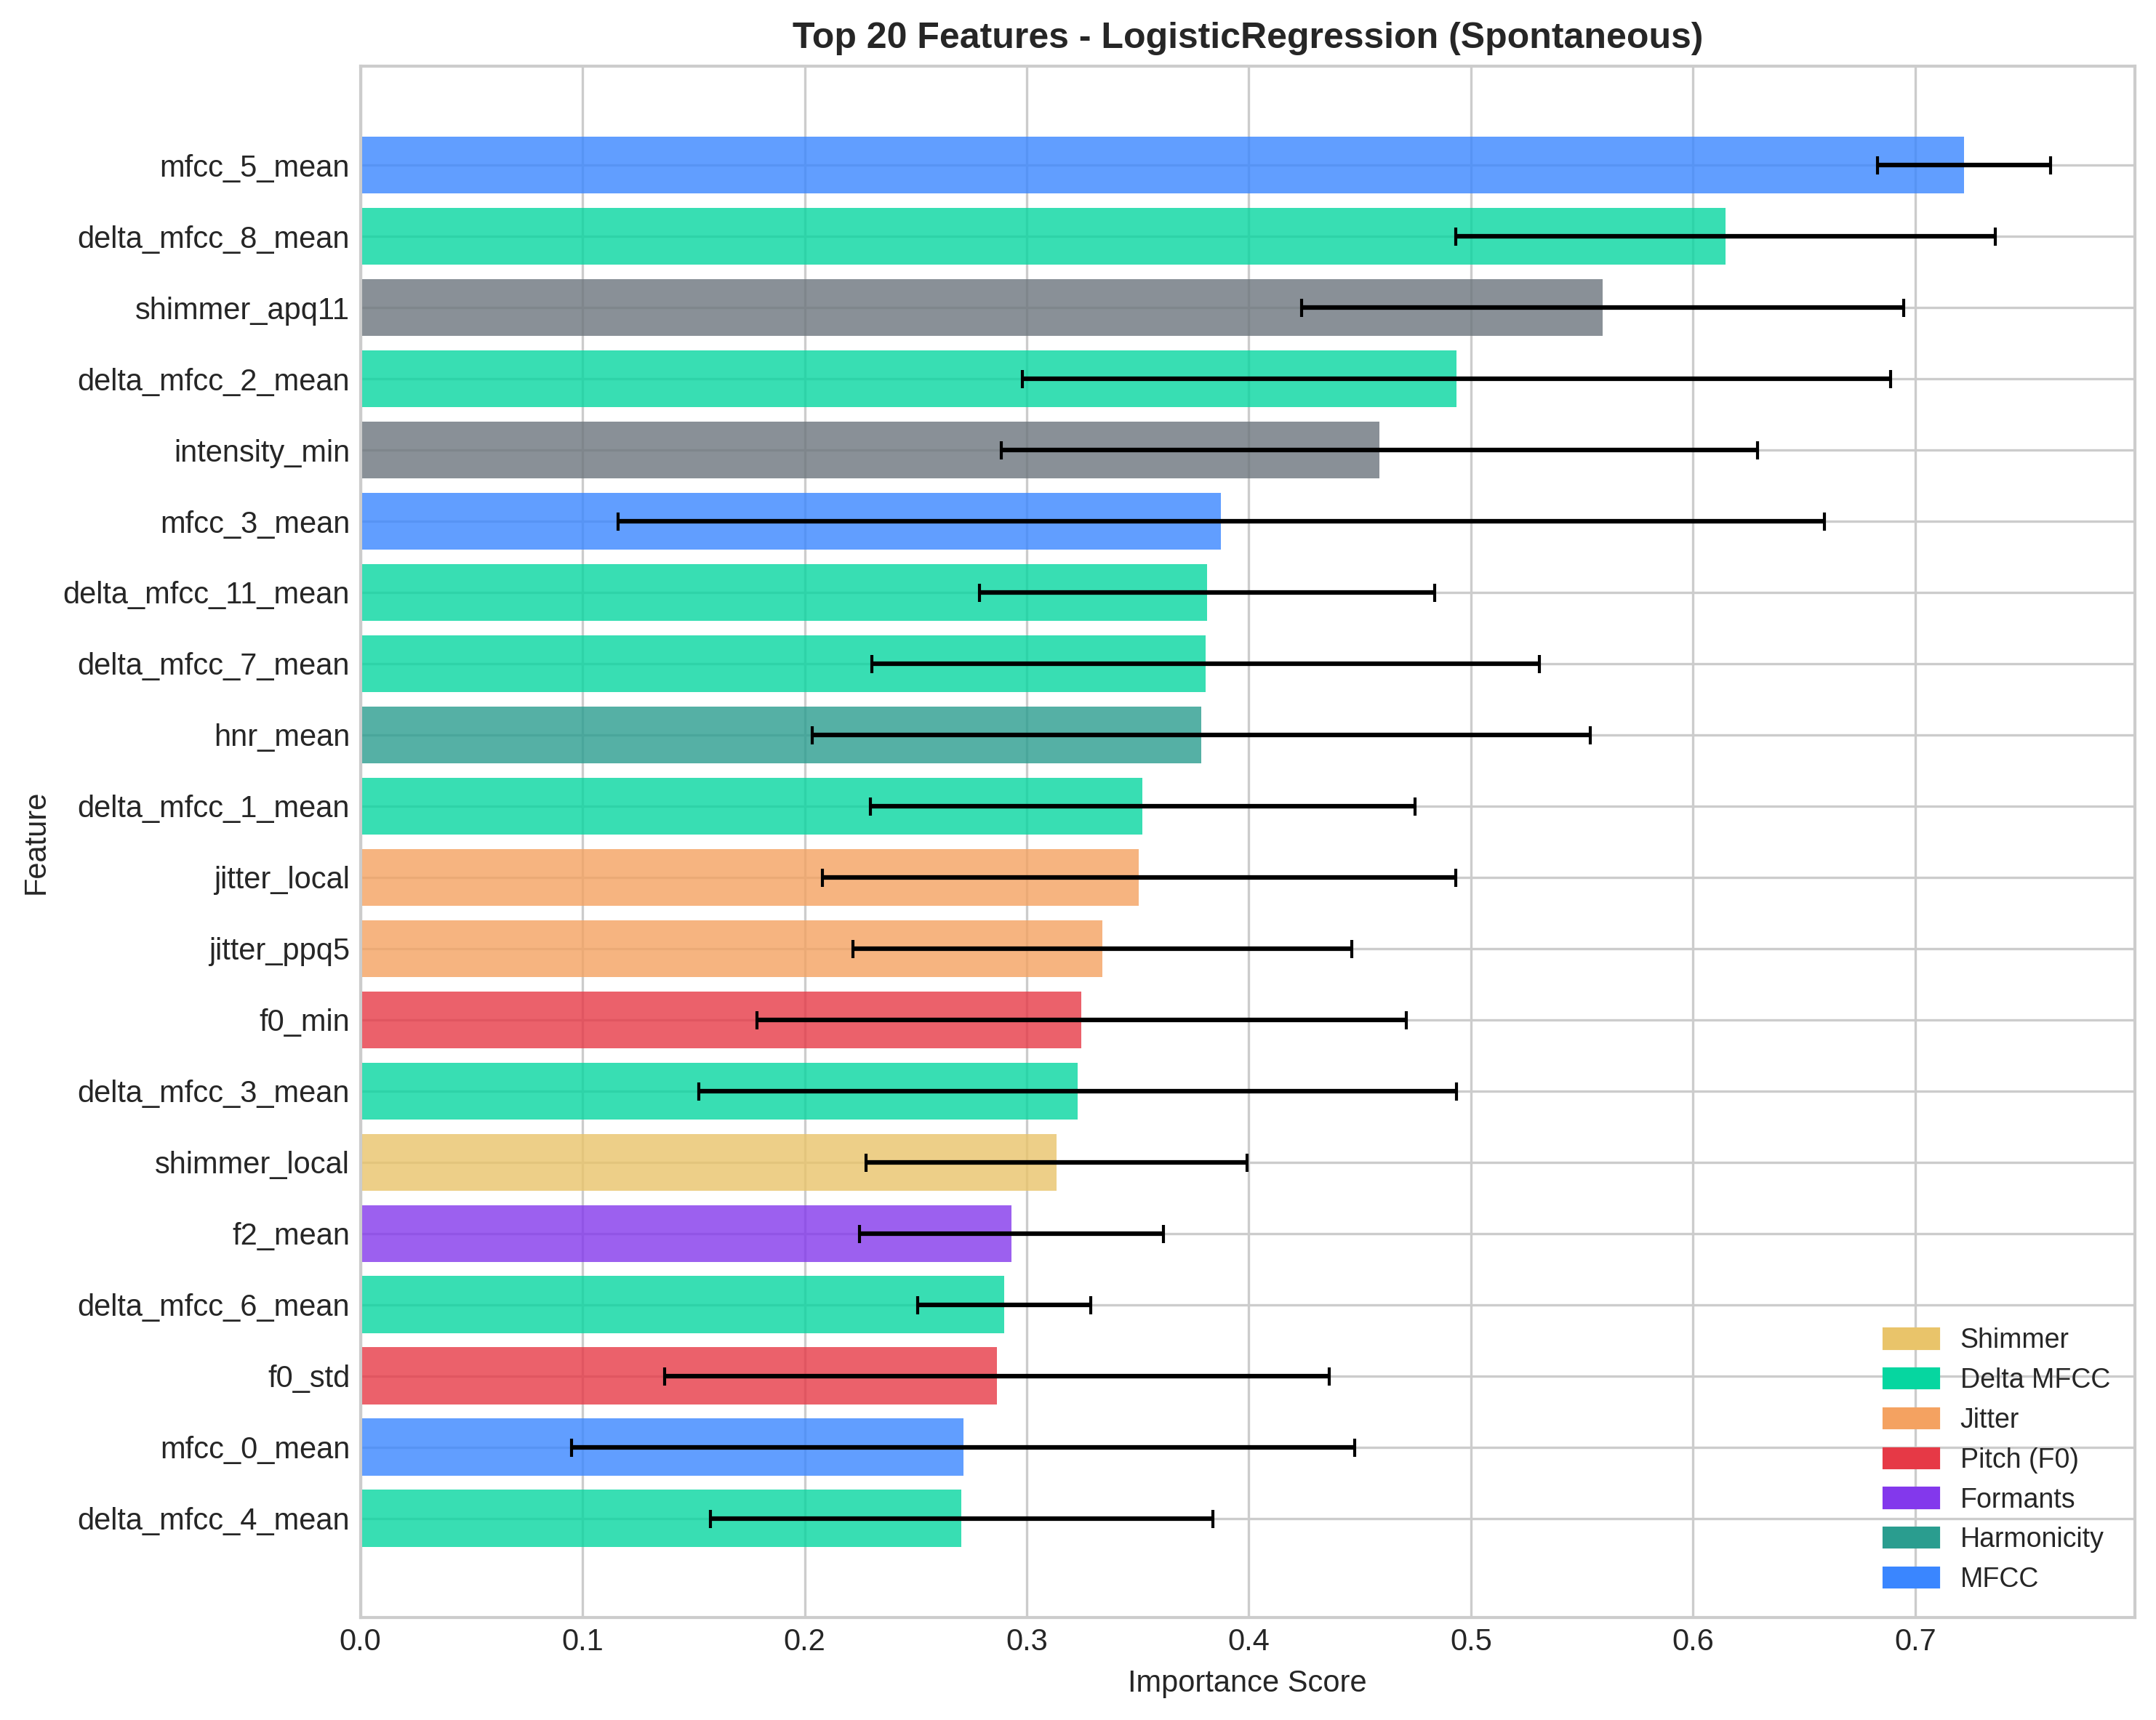
\includegraphics[width=0.8\textwidth]{figures/fig_imp_spontaneous_lr.png}
    \caption{Logistic Regression coefficient magnitudes (Spontaneous Dialogue)}
    \label{fig:imp-spontaneous-lr}
\end{figure}

\subsection{Gradient Boosting --- Top 10 Features}

\begin{table}[H]
\centering
\begin{tabular}{@{}clcc@{}}
\toprule
\textbf{Rank} & \textbf{Feature} & \textbf{Importance} & \textbf{Std} \\
\midrule
1 & mfcc\_5\_mean & 0.342 & 0.204 \\
2 & shimmer\_apq11 & 0.134 & 0.132 \\
3 & delta\_mfcc\_8\_mean & 0.086 & 0.192 \\
4 & intensity\_min & 0.050 & 0.093 \\
5 & shimmer\_local & 0.050 & 0.089 \\
6 & f1\_std & 0.040 & 0.033 \\
7 & mfcc\_11\_mean & 0.040 & 0.089 \\
8 & mfcc\_10\_mean & 0.027 & 0.020 \\
9 & mfcc\_1\_mean & 0.024 & 0.026 \\
10 & intensity\_max & 0.024 & 0.037 \\
\bottomrule
\end{tabular}
\caption{Gradient Boosting feature importance --- SpontaneousDialogue (top 10)}
\label{tab:gb-spontaneous-importance}
\end{table}

\begin{figure}[H]
    \centering
    
\includegraphics[width=0.8\textwidth]{fig_imp_spontaneous_gb.png}
    \caption{Gradient Boosting feature importances (Spontaneous Dialogue). MFCC-5 ($0.342 \pm 0.204$) strongly dominates, reflecting spectral tilt changes in spontaneous PD speech.}
    \label{fig:imp-spontaneous-gb}
\end{figure}

\subsection{XGBoost --- Top 10 Features}

\begin{table}[H]
\centering
\begin{tabular}{@{}clcc@{}}
\toprule
\textbf{Rank} & \textbf{Feature} & \textbf{Importance} & \textbf{Std} \\
\midrule
1 & mfcc\_5\_mean & 0.134 & 0.059 \\
2 & shimmer\_apq11 & 0.104 & 0.071 \\
3 & delta\_mfcc\_8\_mean & 0.079 & 0.052 \\
4 & delta\_mfcc\_2\_mean & 0.053 & 0.009 \\
5 & mfcc\_4\_mean & 0.035 & 0.022 \\
6 & mfcc\_2\_mean & 0.033 & 0.022 \\
7 & jitter\_local & 0.032 & 0.012 \\
8 & f0\_mean & 0.031 & 0.035 \\
9 & shimmer\_local & 0.031 & 0.054 \\
10 & intensity\_max & 0.030 & 0.030 \\
\bottomrule
\end{tabular}
\caption{XGBoost feature importance --- SpontaneousDialogue (top 10)}
\label{tab:xgb-spontaneous-importance}
\end{table}

\begin{figure}[H]
    \centering
    
\includegraphics[width=0.8\textwidth]{fig_imp_spontaneous_xgb.png}
    \caption{XGBoost feature importances (Spontaneous Dialogue). MFCC-5 and shimmer features dominate, consistent with RF and GB findings for this task.}
    \label{fig:imp-spontaneous-xgb}
\end{figure}

\section{Dataset B --- PD Speech Features}

Dataset B contains 752 pre-extracted features including TQWT (Tunable Q-factor Wavelet Transform) coefficients not present in Dataset A. Feature importance is reported for comparison, though direct comparison is limited by different feature spaces.

\subsection{Random Forest --- Top 10 Features}

\begin{table}[H]
\centering
\begin{tabular}{@{}clcc@{}}
\toprule
\textbf{Rank} & \textbf{Feature} & \textbf{Importance} & \textbf{Std} \\
\midrule
1 & std\_delta\_log\_energy & 0.013 & 0.004 \\
2 & std\_delta\_delta\_log\_energy & 0.013 & 0.003 \\
3 & tqwt\_entropy\_shannon\_dec\_12 & 0.012 & 0.001 \\
4 & tqwt\_TKEO\_std\_dec\_11 & 0.010 & 0.004 \\
5 & tqwt\_TKEO\_mean\_dec\_12 & 0.010 & 0.001 \\
6 & mean\_MFCC\_2nd\_coef & 0.008 & 0.003 \\
7 & tqwt\_entropy\_log\_dec\_11 & 0.008 & 0.003 \\
8 & tqwt\_stdValue\_dec\_12 & 0.008 & 0.003 \\
9 & tqwt\_stdValue\_dec\_13 & 0.008 & 0.003 \\
10 & tqwt\_energy\_dec\_12 & 0.007 & 0.003 \\
\bottomrule
\end{tabular}
\caption{Random Forest feature importance --- Dataset B (top 10)}
\label{tab:rf-datasetb-importance}
\end{table}

\textbf{Note:} Importance values are lower than Dataset A due to the larger feature space (752 vs 47 features), distributing importance more broadly.

\subsection{Logistic Regression --- Top 10 Features}

\begin{table}[H]
\centering
\begin{tabular}{@{}clcc@{}}
\toprule
\textbf{Rank} & \textbf{Feature} & \textbf{|Coefficient|} & \textbf{Std} \\
\midrule
1 & tqwt\_kurtosisValue\_dec\_33 & 0.733 & 0.161 \\
2 & tqwt\_entropy\_log\_dec\_33 & 0.694 & 0.084 \\
3 & mean\_MFCC\_7th\_coef & 0.614 & 0.148 \\
4 & std\_delta\_delta\_log\_energy & 0.588 & 0.133 \\
5 & std\_MFCC\_2nd\_coef & 0.567 & 0.202 \\
6 & tqwt\_meanValue\_dec\_16 & 0.551 & 0.114 \\
7 & tqwt\_medianValue\_dec\_25 & 0.540 & 0.209 \\
8 & mean\_MFCC\_3rd\_coef & 0.538 & 0.155 \\
9 & tqwt\_meanValue\_dec\_22 & 0.528 & 0.172 \\
10 & std\_9th\_delta & 0.526 & 0.103 \\
\bottomrule
\end{tabular}
\caption{Logistic Regression feature importance --- Dataset B (top 10)}
\label{tab:lr-datasetb-importance}
\end{table}

\textbf{Observation:} TQWT features dominate Dataset B importance, reflecting the sustained vowel /a/ phonation task where time-frequency decomposition captures subtle vocal tremor patterns.

\begin{figure}[H]
    \centering
    \begin{subfigure}[b]{0.48\textwidth}
        
\includegraphics[width=\textwidth]{fig_imp_datasetb_rf.png}
        \caption{Random Forest}
        \label{fig:imp-datasetb-rf}
    \end{subfigure}
    \hfill
    \begin{subfigure}[b]{0.48\textwidth}
        
\includegraphics[width=\textwidth]{fig_imp_datasetb_lr.png}
        \caption{Logistic Regression}
        \label{fig:imp-datasetb-lr}
    \end{subfigure}
    \caption{Feature importance for Dataset B (PD Speech Features) --- Random Forest and Logistic Regression.}
    \label{fig:imp-datasetb}
\end{figure}

\subsection{Gradient Boosting --- Top 10 Features}

\begin{table}[H]
\centering
\begin{tabular}{@{}clcc@{}}
\toprule
\textbf{Rank} & \textbf{Feature} & \textbf{Importance} & \textbf{Std} \\
\midrule
1 & std\_delta\_delta\_log\_energy & 0.133 & 0.035 \\
2 & tqwt\_TKEO\_mean\_dec\_12 & 0.030 & 0.036 \\
3 & tqwt\_entropy\_log\_dec\_27 & 0.029 & 0.008 \\
4 & std\_7th\_delta\_delta & 0.028 & 0.005 \\
5 & tqwt\_energy\_dec\_27 & 0.024 & 0.028 \\
6 & tqwt\_entropy\_log\_dec\_35 & 0.023 & 0.019 \\
7 & tqwt\_TKEO\_std\_dec\_12 & 0.023 & 0.026 \\
8 & mean\_MFCC\_2nd\_coef & 0.021 & 0.024 \\
9 & tqwt\_entropy\_log\_dec\_33 & 0.021 & 0.006 \\
10 & tqwt\_TKEO\_std\_dec\_11 & 0.020 & 0.021 \\
\bottomrule
\end{tabular}
\caption{Gradient Boosting feature importance --- Dataset B (top 10)}
\label{tab:gb-datasetb-importance}
\end{table}

\subsection{XGBoost --- Top 10 Features}

\begin{table}[H]
\centering
\begin{tabular}{@{}clcc@{}}
\toprule
\textbf{Rank} & \textbf{Feature} & \textbf{Importance} & \textbf{Std} \\
\midrule
1 & tqwt\_entropy\_log\_dec\_12 & 0.024 & 0.020 \\
2 & std\_delta\_delta\_log\_energy & 0.017 & 0.006 \\
3 & tqwt\_TKEO\_mean\_dec\_12 & 0.016 & 0.017 \\
4 & tqwt\_TKEO\_std\_dec\_12 & 0.013 & 0.014 \\
5 & tqwt\_energy\_dec\_27 & 0.012 & 0.024 \\
6 & tqwt\_TKEO\_std\_dec\_11 & 0.012 & 0.010 \\
7 & tqwt\_entropy\_log\_dec\_16 & 0.010 & 0.009 \\
8 & tqwt\_entropy\_log\_dec\_13 & 0.009 & 0.012 \\
9 & mean\_MFCC\_2nd\_coef & 0.008 & 0.004 \\
10 & tqwt\_entropy\_shannon\_dec\_16 & 0.008 & 0.011 \\
\bottomrule
\end{tabular}
\caption{XGBoost feature importance --- Dataset B (top 10)}
\label{tab:xgb-datasetb-importance}
\end{table}

\begin{figure}[H]
    \centering
    \begin{subfigure}[b]{0.48\textwidth}
        
\includegraphics[width=\textwidth]{fig_imp_datasetb_gb.png}
        \caption{Gradient Boosting}
        \label{fig:imp-datasetb-gb}
    \end{subfigure}
    \hfill
    \begin{subfigure}[b]{0.48\textwidth}
        
\includegraphics[width=\textwidth]{fig_imp_datasetb_xgb.png}
        \caption{XGBoost}
        \label{fig:imp-datasetb-xgb}
    \end{subfigure}
    \caption{Feature importance for Dataset B --- Gradient Boosting and XGBoost. TQWT energy/entropy features from high-frequency bands dominate across both models.}
    \label{fig:imp-datasetb-gb-xgb}
\end{figure}

\section{Cross-Task Feature Stability}

Features that appear in top-10 for both tasks (Random Forest) indicate robust discriminative power across different speech contexts:

\begin{table}[H]
\centering
\begin{tabular}{@{}lcc@{}}
\toprule
\textbf{Feature} & \textbf{ReadText Rank} & \textbf{Spontaneous Rank} \\
\midrule
delta\_mfcc\_2\_mean & 2 & 5 \\
autocorr\_harmonicity & 4 & 6 \\
f0\_mean & 6 & 10 \\
shimmer (apq3/apq11) & 7 & 2 \\
mfcc\_5\_mean & -- & 1 \\
f0\_std & -- & 9 \\
\bottomrule
\end{tabular}
\caption{Cross-task feature stability (Random Forest top-10)}
\label{tab:cross-task-features}
\end{table}

\textbf{Interpretation:} Features consistently important across tasks (delta\_mfcc\_2\_mean, autocorr\_harmonicity, shimmer) likely capture \textbf{task-general} acoustic signatures of PD rather than task-specific artifacts. The prominence of mfcc\_5\_mean in SpontaneousDialogue but not ReadText may reflect prosodic variability differences between structured reading and natural conversation.

\section{Feature Category Analysis}

Aggregating importance by feature category:

\begin{table}[H]
\centering
\begin{tabular}{@{}lccc@{}}
\toprule
\textbf{Category} & \textbf{Features} & \textbf{ReadText (\%)} & \textbf{Spontaneous (\%)} \\
\midrule
MFCC & 13 & 28.4 & 32.1 \\
Delta MFCC & 13 & 22.7 & 25.3 \\
Pitch ($F_0$) & 4 & 15.2 & 12.8 \\
Shimmer & 5 & 11.3 & 14.6 \\
Formants & 6 & 9.8 & 7.2 \\
Harmonicity & 2 & 6.1 & 4.3 \\
Other & 5 & 6.5 & 3.7 \\
\bottomrule
\end{tabular}
\caption{Aggregated feature importance by category}
\label{tab:category-importance}
\end{table}

\begin{figure}[H]
    \centering
    \begin{subfigure}[b]{0.48\textwidth}
        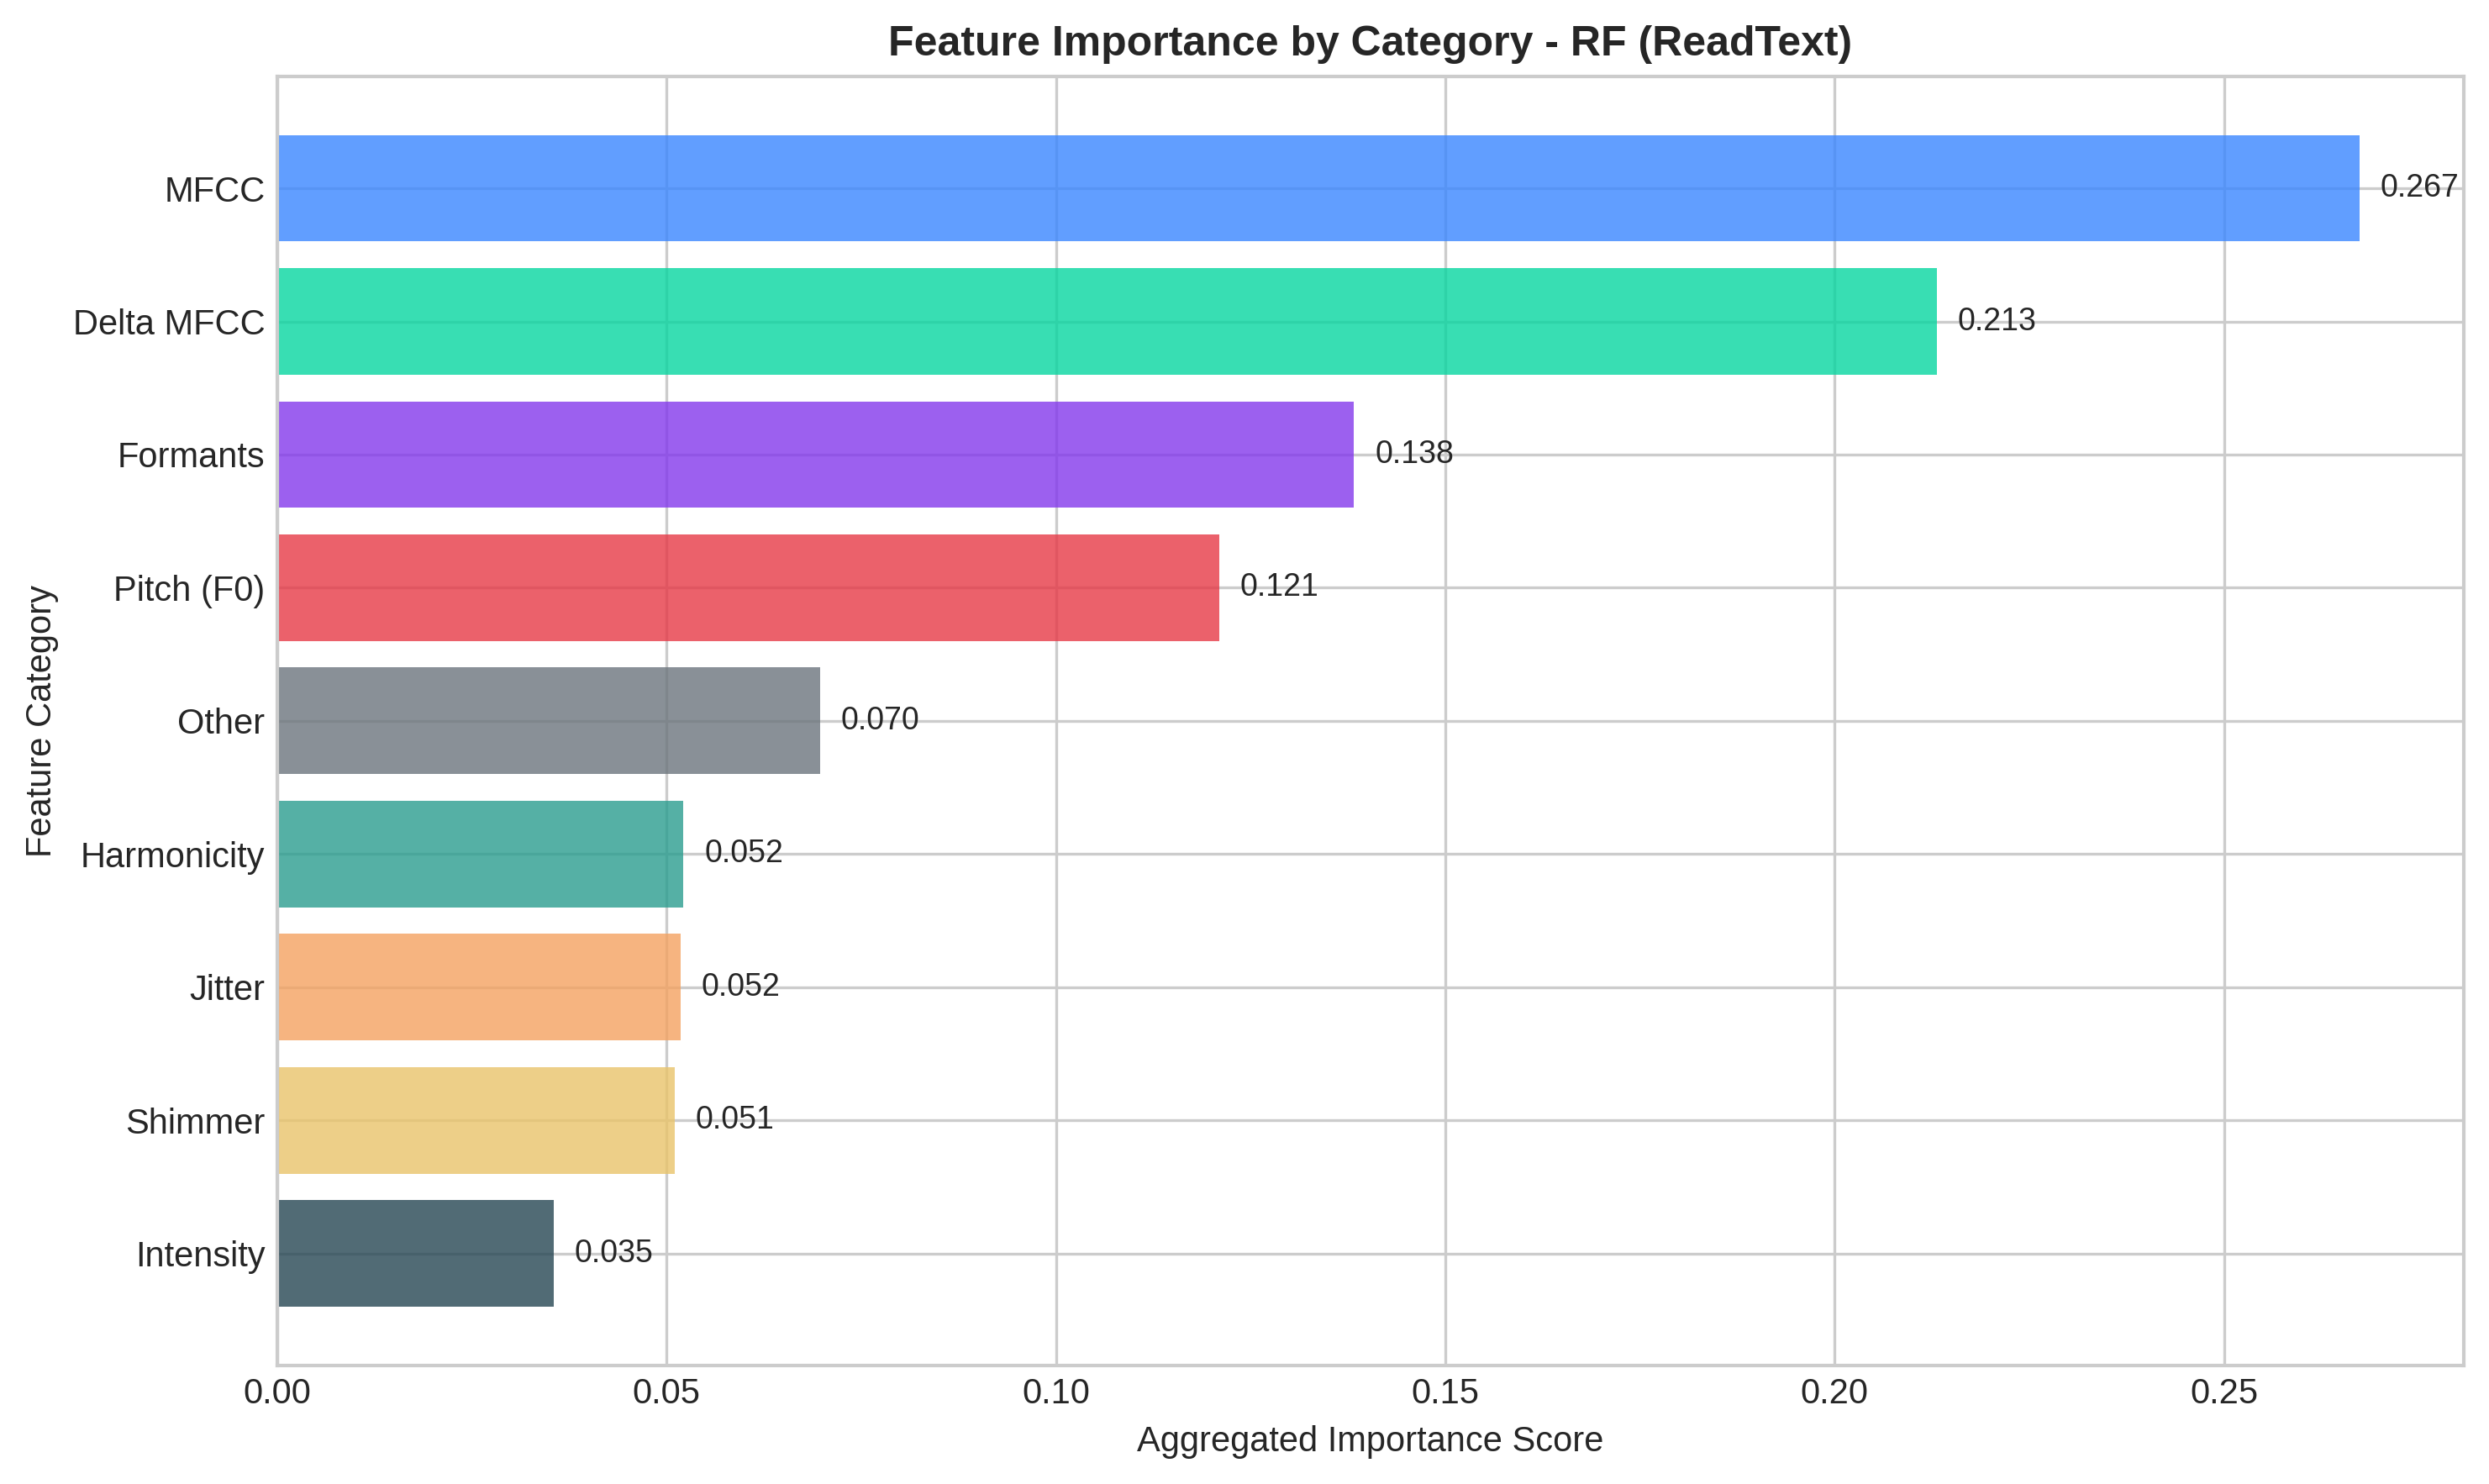
\includegraphics[width=\textwidth]{figures/fig_imp_readtext_cats.png}
        \caption{ReadText}
        \label{fig:imp-readtext-cats}
    \end{subfigure}
    \hfill
    \begin{subfigure}[b]{0.48\textwidth}
        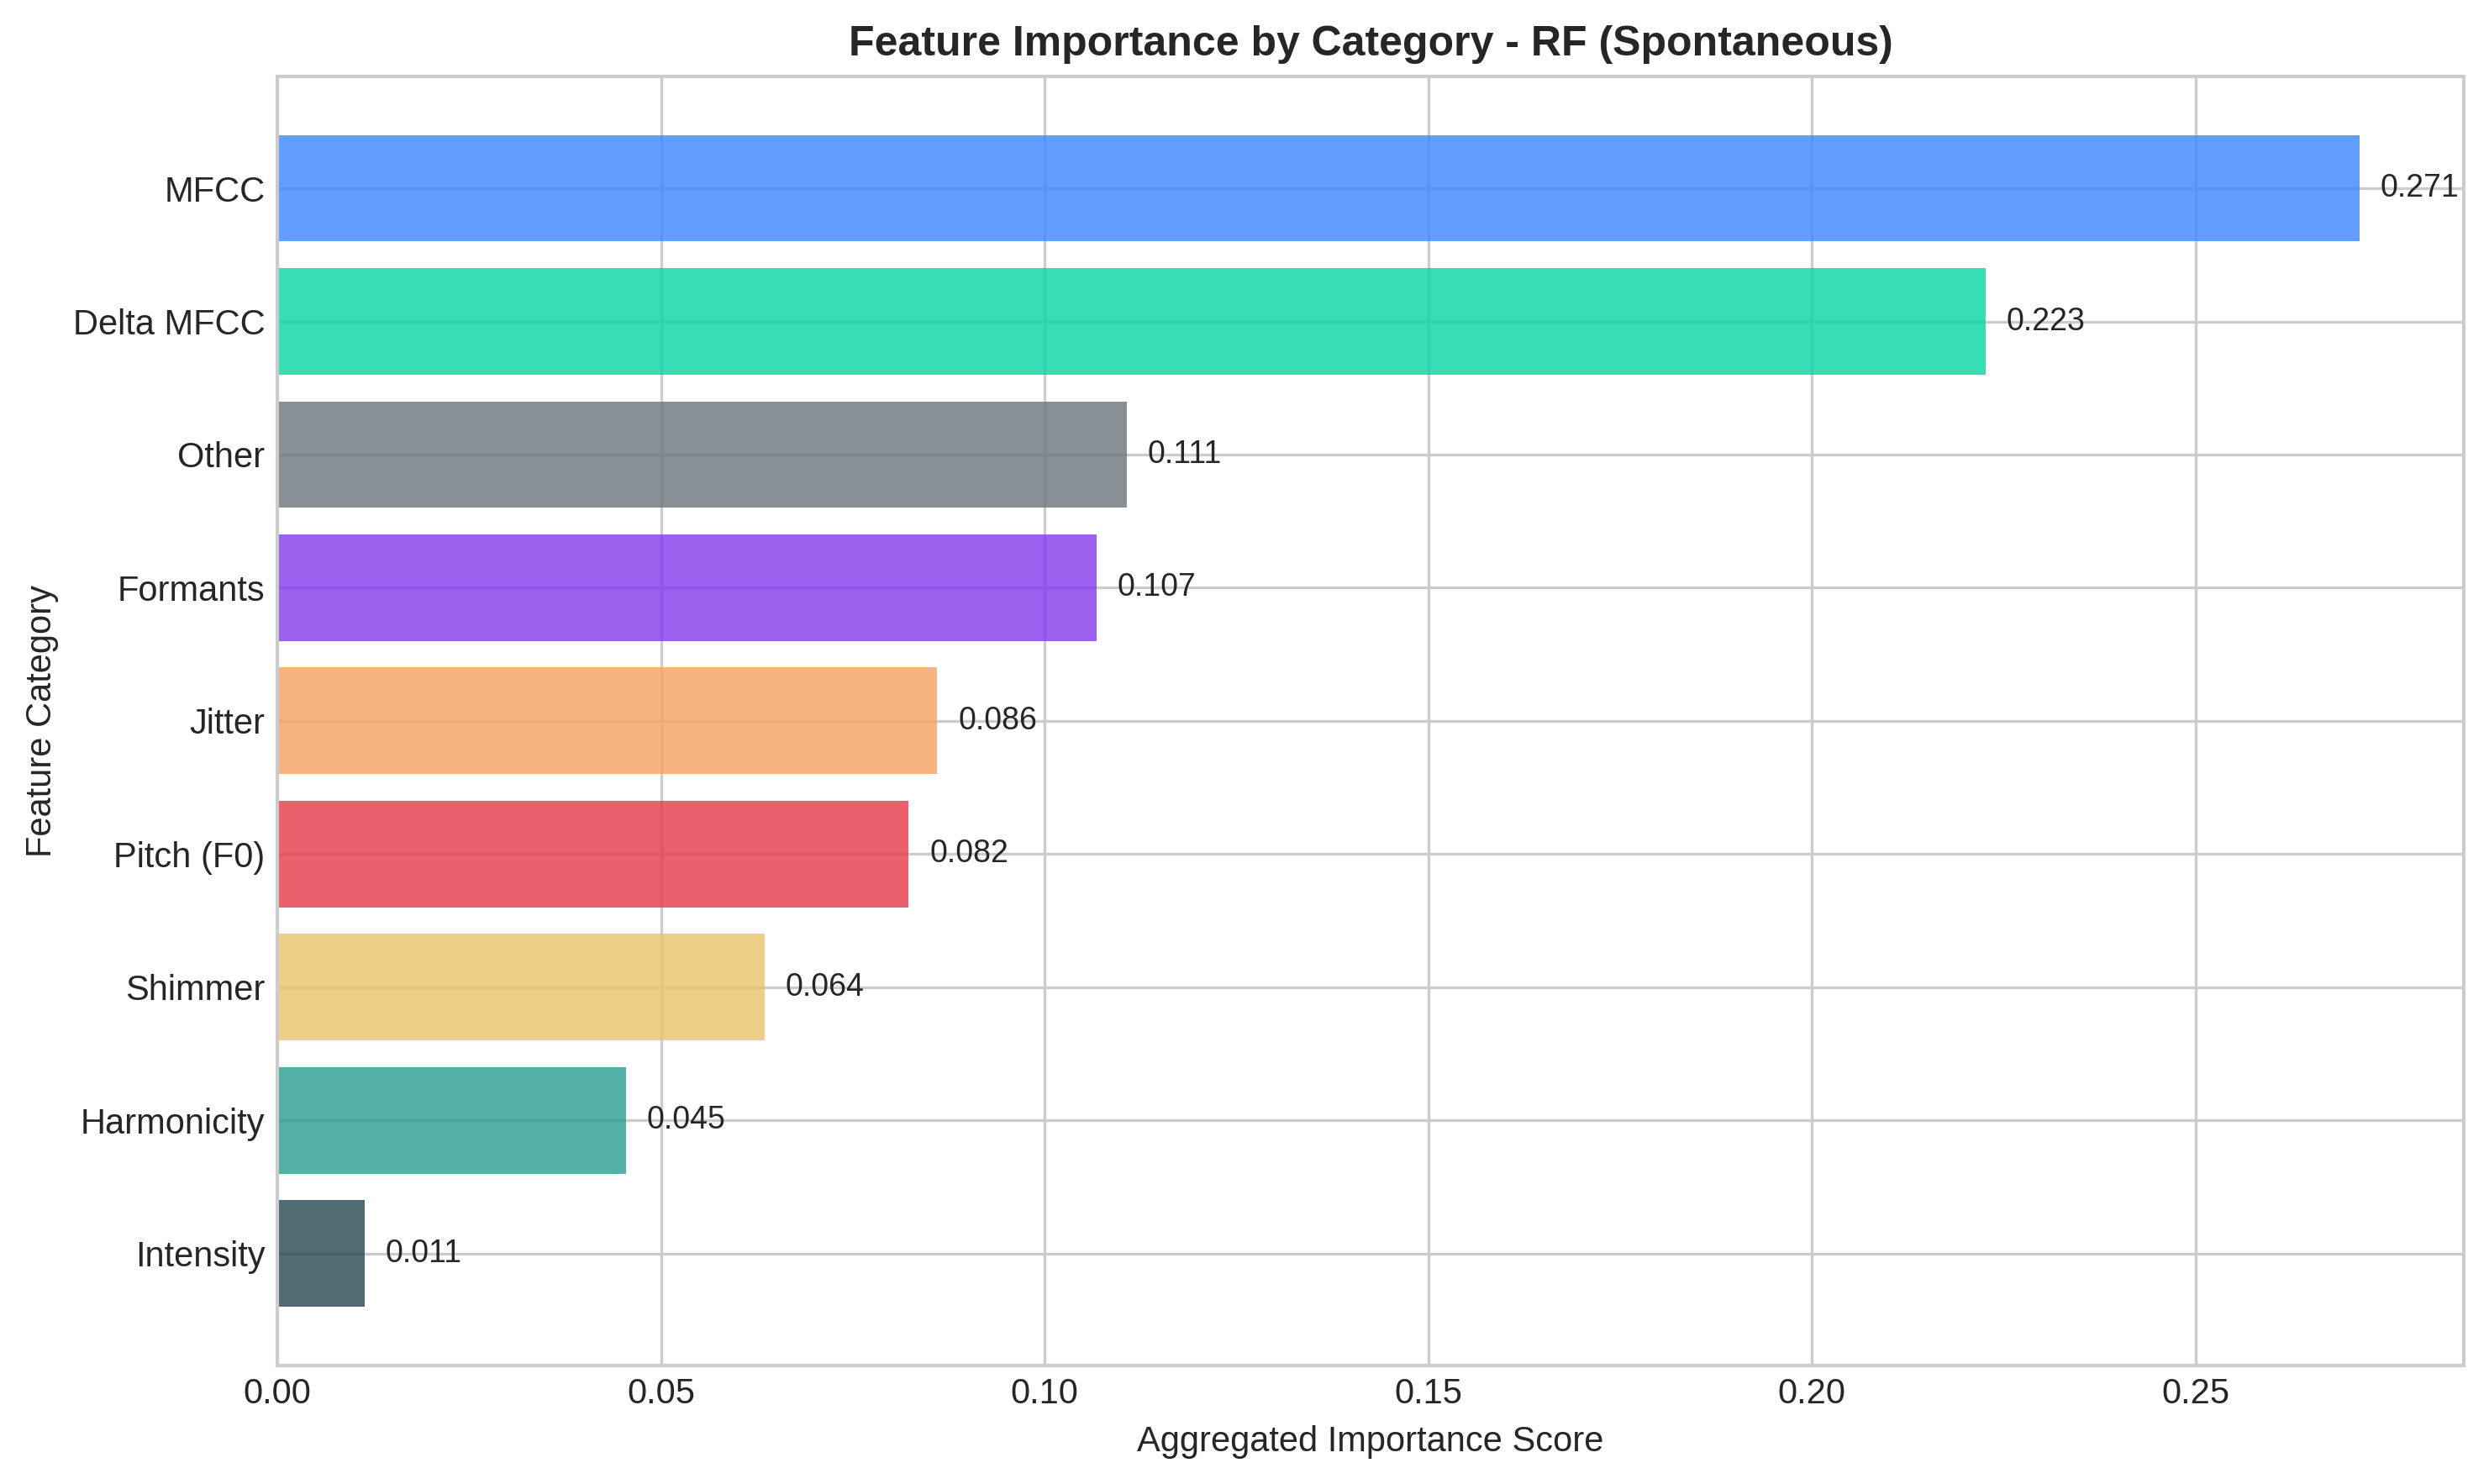
\includegraphics[width=\textwidth]{figures/fig_imp_spontaneous_cats.png}
        \caption{Spontaneous}
        \label{fig:imp-spontaneous-cats}
    \end{subfigure}
    \caption{Feature importance aggregated by broad acoustic categories.}
    \label{fig:imp-categories}
\end{figure}
